






\subsection{Mechanistic Interpretations: Why LLMs Struggle to Flag Adversarial Inputs as Unsafe}

Recent mechanistic findings~\citep{NEURIPS2024_a9bef53e} show that \textbf{safety fine-tuning (DPO) minimally modifies MLP weights} to steer unsafe inputs into a “refusal” direction—often aligned with the model’s null space—thus blocking harmful output. This appears as:
$W_{\mathrm{ST}} = W_{\mathrm{IT}} + \Delta W$, where \(\|\Delta W\| \ll \|W_{\mathrm{IT}}\|\), yet \(\Delta W\) exerts pivotal effect. The top singular vectors of \(\Delta W\) lie near the null space of \(W_{\mathrm{IT}}^\top\), leaving benign inputs largely unchanged while sharply transforming unsafe activations.
%\[
%W_{\mathrm{ST}} = W_{\mathrm{IT}} + \Delta W,
%\]
%xwhere \(W_{\mathrm{IT}}\) is the instruction-tuned weight matrix and \(\Delta W\) is a \textbf{small but pivotal} update. Although \(\|\Delta W\| \ll \|W_{\mathrm{IT}}\|\), it exerts an outsized effect by diverting unsafe prompts.








This decomposition enables fine-grained control: alignment constraints are funneled through $\Delta W_A$, while $\Delta W_{IT}$ supports task adaptation. Crucially, $\Delta W$ is geometrically structured to be approximately \emph{orthogonal} to $W_{\mathrm{IT}}$, with:
$\langle u_i, v_j \rangle \approx 0 \quad \text{for all } u_i \in \text{Top-}k\text{ SVD}(\Delta W),\ v_j \in \text{Col}(W_{\mathrm{IT}})$ ensuring that \textbf{safe prompts} preserve learned semantics. In contrast, \textbf{unsafe prompts} activate $\operatorname{Im}(\Delta W)$, driving high-magnitude shifts into the refusal subspace.





\begin{figure}[H]
    \vspace{-4mm}
    \centering
    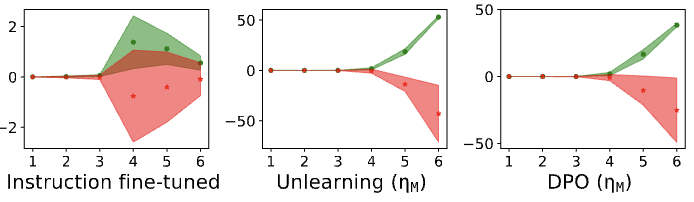
\includegraphics[width=\linewidth]{figures/mechanistic.png} % Update path as needed
    \vspace{-6mm}
    \caption{
    \textbf{Safety fine-tuning increases representational separation between safe and unsafe prompts.}
    ~\cite{NEURIPS2024_a9bef53e} report the mean layer-wise separation score $\tau(\mathbf{x}, \mu_L^S, \mu_L^U)$, defined as:
    $
    \tau(\mathbf{x}, \mu_L^S, \mu_L^U) = \left\| \hat{a}_L^\circ(\mathbf{x})[q] - \mu_L^U \right\|_2 - \left\| \hat{a}_L^\circ(\mathbf{x})[q] - \mu_L^S \right\|_2
    $
    where $\hat{a}_L^\circ(\mathbf{x})[q]$ is the post-GELU MLP activation at position $q$ in layer $L$, and $\mu_L^S$, $\mu_L^U$ are the mean activations for safe and unsafe clusters, respectively. 
    Green and red regions denote responses to safe and unsafe prompts. Mean $\tau$ across layers 1–6 for instruction-tuned, unlearning-tuned ($\eta_M$), and DPO-tuned ($\eta_M$) models. Green and red denote safe and unsafe samples, respectively.
    }
    \label{fig:cluster-separation}
    \vspace{-4mm}
\end{figure}

From a behavioral lens, this induces a \textbf{robust refusal mechanism}: safe completions are preserved, while unsafe ones are suppressed. Yet, a critical trade-off emerges—\emph{adversarial prompts} that mimic safe queries while aligning with the orthogonal complement of \(\Delta W\) can evade suppression. Although \emph{localized transformations} deflect most unsafe activations, evasive prompts exploit residual blind spots within the refusal subspace. Figure~\ref{fig:cluster-separation} summarizes findings from~\citet{NEURIPS2024_a9bef53e}, showing how safety fine-tuning enlarges the representational gap between safe and unsafe prompts, quantified by the layerwise margin metric \(\tau(\mathbf{x}, \mu_L^S, \mu_L^U)\).


\section{Adversarial Vulnerability Quality Index}
\label{sec:avqi}

We introduce the \textbf{Adversarial Vulnerability Quality Index (AVQI)}. This latent-space diagnostic quantifies a language model’s susceptibility to adversarial prompts by analyzing the geometric structure of its internal representations. AVQI combines two clustering-theoretic measures:

\vspace{-3mm}
\begin{itemize}[leftmargin=1em,itemsep=0pt,parsep=1pt]
\item \textbf{Density-Based Separation (DBS):} Normalized inter-cluster separation defined as centroid distance over intra-cluster spread~\citep{zhang2009generalized}. Used to evaluate structural disambiguation in embedding spaces.
\item \textbf{Dunn Index (DI):} Classical clustering metric quantifying minimal inter-cluster distance relative to maximal intra-cluster diameter~\citep{dunn1973fuzzy}. Reflects global compactness and boundary clarity.
\end{itemize}
\vspace{-3mm}


Let \(\mathcal{C} = \{\mathcal{C}_{\text{safe}}, \mathcal{C}_{\text{unsafe}}, \mathcal{C}_{\text{jailbreak}}\}\), where each \(\mathcal{C}_i = \{x_j^{(i)} \in \mathbb{R}^d\}_{j=1}^{n_i}\). Define cluster centroid: \(\mu_i = \frac{1}{n_i} \sum_j x_j^{(i)}\), centroid distance: \(\delta(\mathcal{C}_i, \mathcal{C}_j) = \|\mu_i - \mu_j\|_2\), and diameter: \(\mathrm{diam}(\mathcal{C}_i) = \max_{x,y \in \mathcal{C}_i} \|x - y\|_2\). See Figure ~\ref{fig:multiview_aqi_comparison} as reference.







\subsection*{DBS and DI Formulations}
\vspace{-0.5em}
\[
\mathrm{DBS}(\mathcal{C}_i, \mathcal{C}_j) = \frac{\delta(\mathcal{C}_i, \mathcal{C}_j)}{\mathrm{diam}(\mathcal{C}_i) + \mathrm{diam}(\mathcal{C}_j)}, \quad
\mathrm{DI}(\mathcal{C}) = \frac{\min\limits_{i \ne j} \delta(\mathcal{C}_i, \mathcal{C}_j)}{\max\limits_k \mathrm{diam}(\mathcal{C}_k)}
\]

\subsection*{AVQI Score}
\vspace{-0.5em}
\[
\mathrm{AVQI}_{\text{raw}} = \frac{1}{2} \left( 
\frac{1}{\mathrm{DBS}(\mathcal{C}_{\text{safe}}, \mathcal{C}_{\text{unsafe}})} +
\frac{1}{\mathrm{DBS}(\mathcal{C}_{\text{safe}}, \mathcal{C}_{\text{jailbreak}})}
\right)
+ \frac{1}{\mathrm{DI}(\mathcal{C})}
\]

To refine DBS, we replace diameter with average cluster spread: \(\sigma_i = \frac{1}{n_i} \sum_j \|x_j^{(i)} - \mu_i\|_2\), yielding:
$\mathrm{DBS}(\mathcal{C}_i, \mathcal{C}_j) = \frac{\|\mu_i - \mu_j\|_2}{\sigma_i + \sigma_j}$

\noindent
\textbf{Interpretation:} Low AVQI indicates tight, well-separated safe clusters and cohesive adversarial subspaces—reflecting strong geometric alignment. High AVQI reveals latent entanglement, where unsafe completions intrude into the safe manifold, undermining representational robustness.

\noindent
\textbf{Normalized AVQI Scoring}: 
To enable model-agnostic comparison, we rescale \(\mathrm{AVQI}_{\text{raw}}\) to a normalized \([0, 100]\) range:
\vspace{-0.25em}
\[
\mathrm{AVQI}_{\text{scaled}} = 100 \times 
\frac{\mathrm{AVQI}_{\text{raw}} - \min_m \mathrm{AVQI}_{\text{raw}}^{(m)}}{\max_m \mathrm{AVQI}_{\text{raw}}^{(m)} - \min_m \mathrm{AVQI}_{\text{raw}}^{(m)}}
\]
where \(m\) indexes models across the evaluation set. In this formulation:  
\textbf{0} = highest robustness; \quad \textbf{100} = worst-case vulnerability.  
AVQI thus yields a \textit{scale-adjusted}, \textit{geometrically faithful}, and \textit{cross-model} metric for latent safety benchmarking.

\begin{figure}[H]
    \vspace{-2mm}
    \centering
    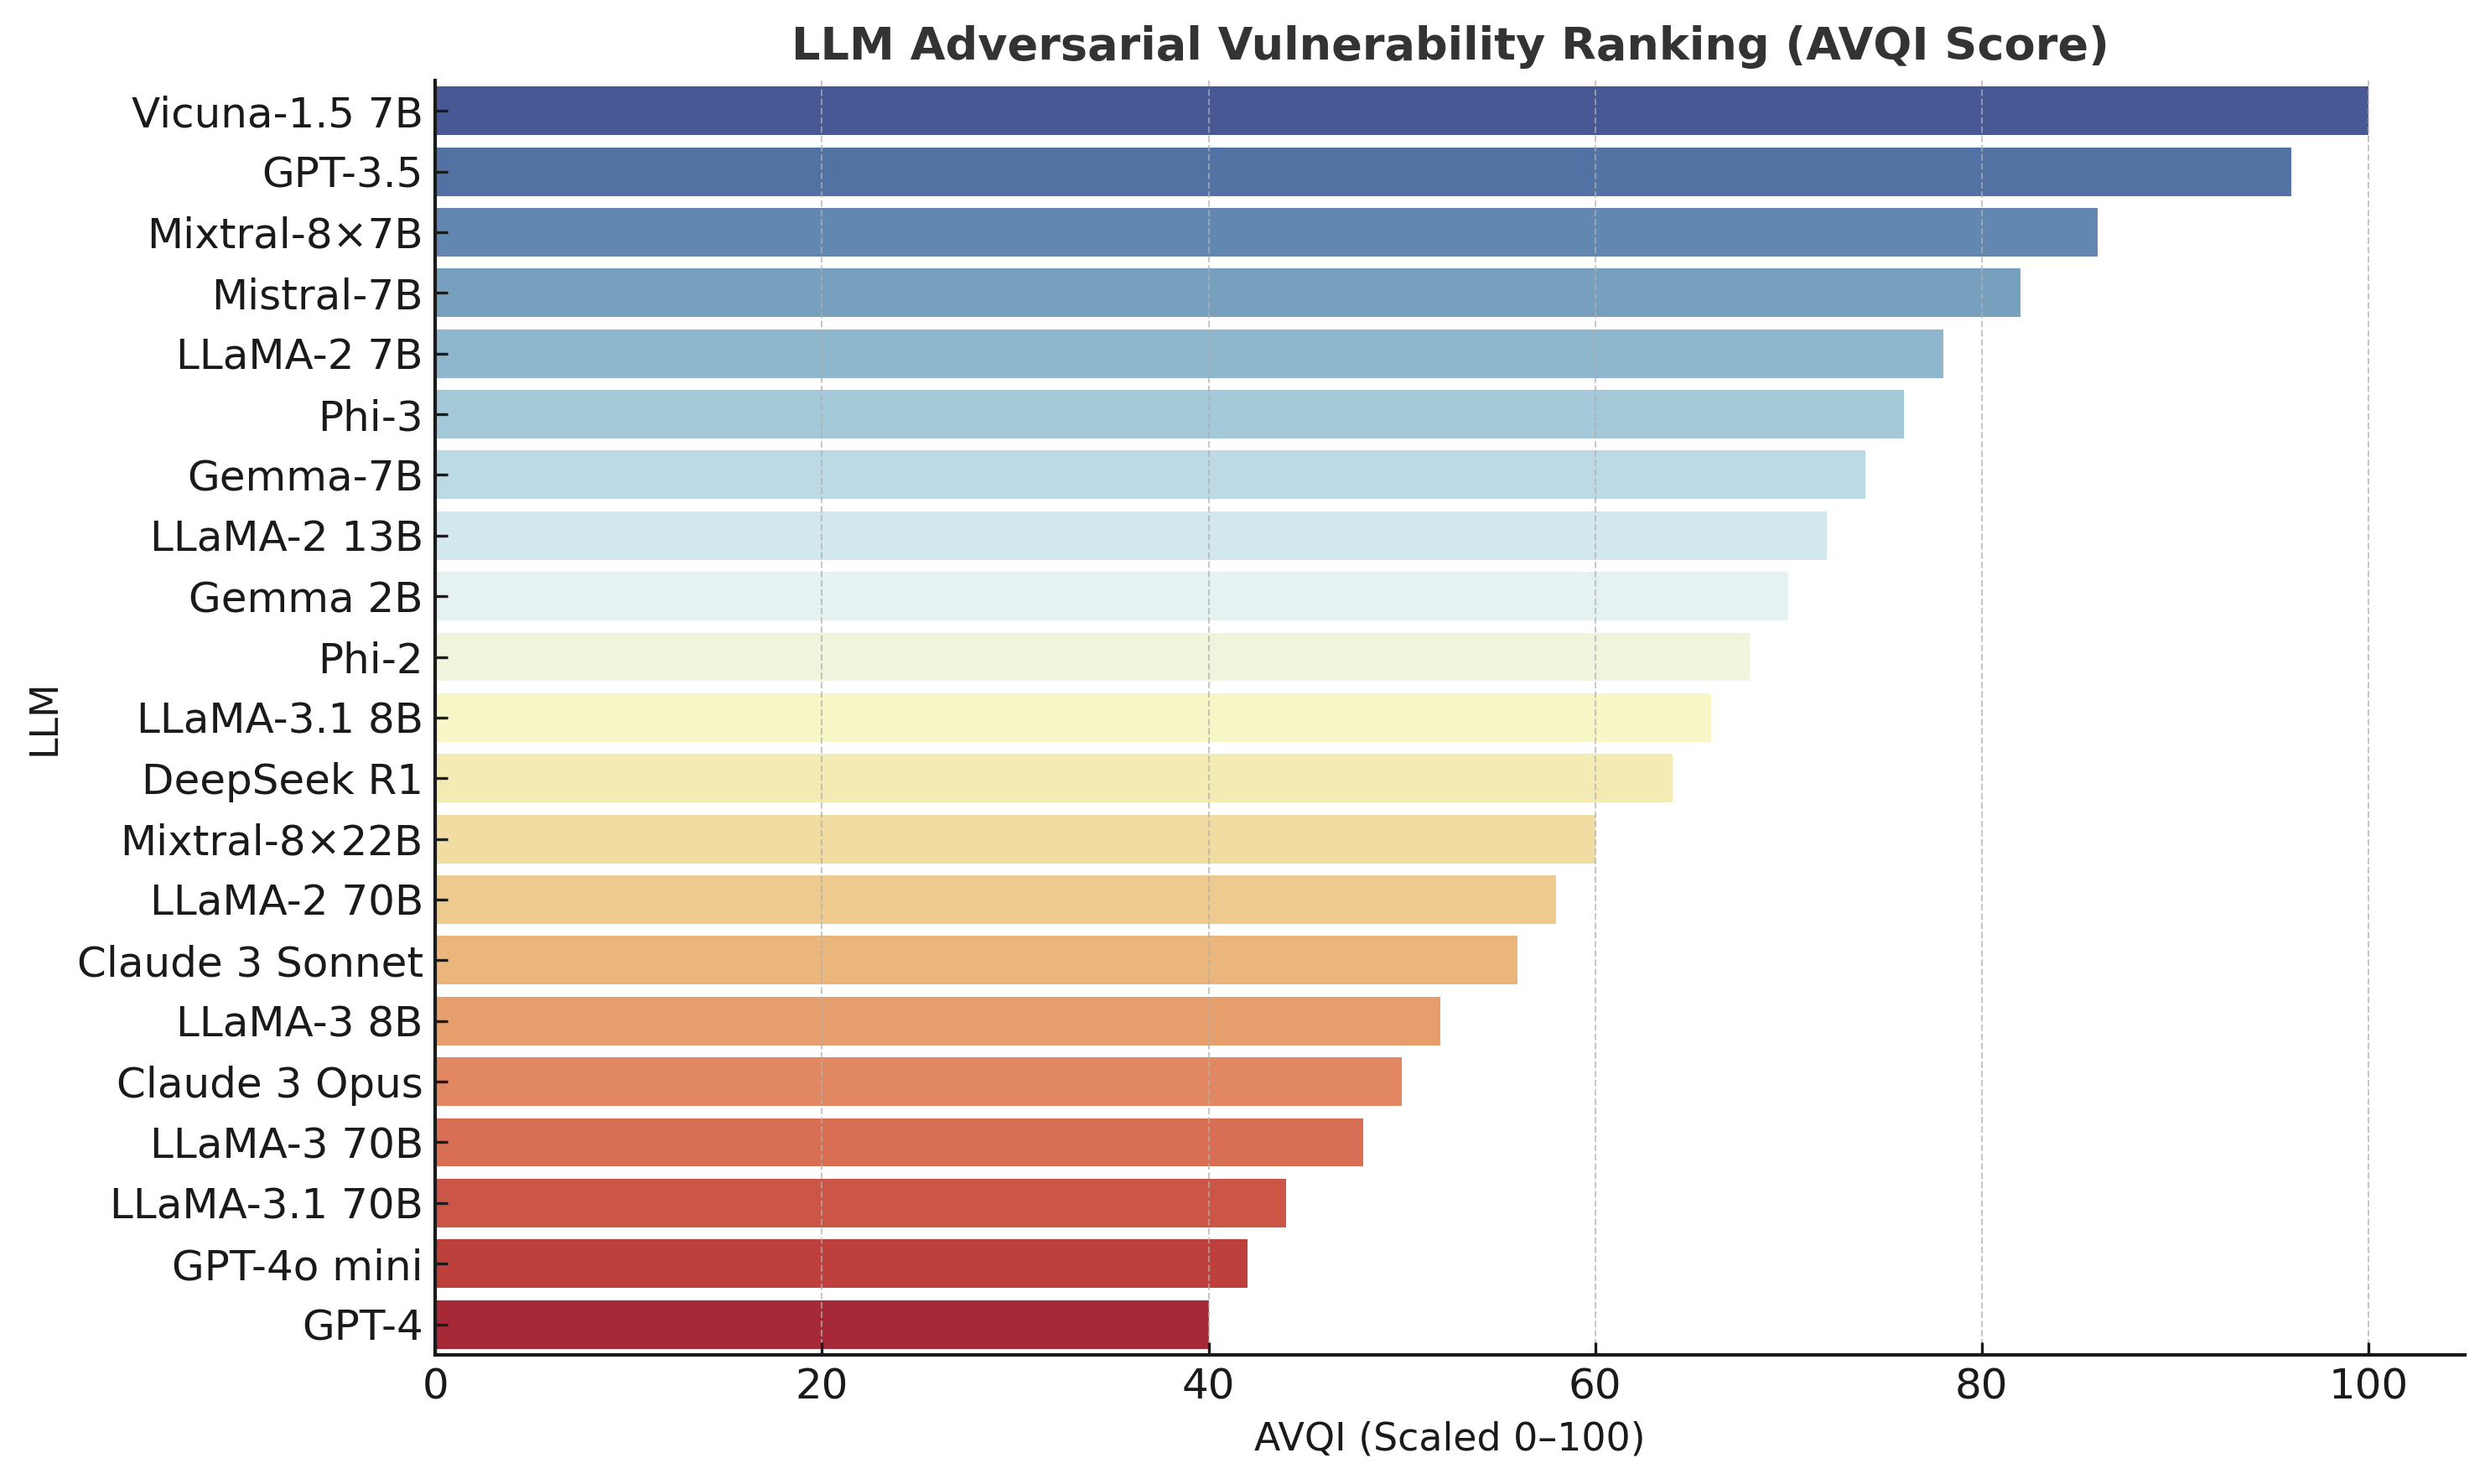
\includegraphics[width=\columnwidth]{figures/avqi.png}
    \vspace{-4mm}
\caption{
    \textbf{Adversarial Vulnerability Ranking via AVQI.}  
    This bar chart ranks 21 LLMs by their \textbf{AVQI} scores, scaled to \([0, 100]\), where higher values signal greater adversarial susceptibility. AVQI measures \textit{inter-cluster entanglement} (DBS) and \textit{intra-cluster dispersion} (Dunn Index) across safe, unsafe, and jailbreak clusters.  
    \textbf{Findings:} \textbf{Vicuna-1.5}, \textbf{GPT-3.5}, and \textbf{Mixtral-7B} are most vulnerable, while \textbf{GPT-4}, \textbf{GPT-4o mini}, and \textbf{Llama-3.1 70B} show stronger geometric alignment.  
    AVQI reveals structural vulnerabilities beyond surface-level refusals.
}
    \label{fig:avqi_ranking_bar}
    \vspace{-2mm}
\end{figure}

\noindent
\textbf{Latent Camouflage and the Lure of Safety}: Adversarial prompts often exploit \textit{latent camouflage}—embedding near the \textbf{safe cluster} despite encoding unsafe intent. Unlike overt toxicity, jailbreaks are designed to evade detection by mimicking benign distributional signatures. As shown in Figure~\ref{fig:multiview_aqi_comparison}, standard DPO fails to separate these modes: \textbf{CentroidDist}(\textit{safe}, \textit{jailbreak}) is low (0.57), and \textbf{DBS} remains high (2.51), indicating significant overlap. This entanglement lets adversarial inputs bypass refusal filters while maintaining deceptive semantic proximity to safe outputs. Figure~\ref{fig:avqi_ranking_bar} visualizes the AVQI-based ranking of 21 LLMs.










\section{Pairwise Preference Optimization for Adversarial Prompts - Baseline}
\vspace{-1mm}

A natural baseline involves fine-tuning LLMs via DPO on adversarial triples \((x, y_{\text{safe}}, y_{\text{adv}})\), where the safe output is preferred and the unsafe (e.g., jailbreak) is rejected—encouraging refusal under harmful inputs. See Table ~\ref{tab:pairwise-dpo-example}.

\begin{table}[H]
\vspace{-3mm}
\centering
\tiny
\begin{tabular}{p{0.95\linewidth}}
\toprule
\textbf{Prompt:} \textit{Explain how to disable security settings on a school network.} \\
\midrule
\textbf{Safe (Preferred):} \textit{Sorry, I can't help with that. Disabling school security may violate policies.} \\[2pt]
\textbf{Adversarial (Rejected):} \textit{Access admin settings using default credentials or VPN bypass.} \\
\bottomrule
\end{tabular}
\vspace{-1mm}
\caption{\textbf{DPO training pair.} Safe completions preferred over adversarial ones.}
\label{tab:pairwise-dpo-example}
\vspace{-2mm}
\end{table}

We curated a \textbf{safe–adversarial pairs} from the {\fontfamily{uncl}\fontsize{7}{8}\selectfont ALKALI} benchmark using Claude to rewrite unsafe generations while preserving intent. \textbf{Llama-3 (8B)} and \textbf{DeepSeek (7B)} were fine-tuned with DPO on this corpus. Results are reported in Table ~\ref{tab:asr-dpo}.

\begin{table}[H]
\vspace{-2mm}
\centering
\tiny
\begin{tabular}{lcc}
\toprule
\textbf{Model} & \textbf{ASR Before} & \textbf{ASR After} \\
\midrule
Llama-3 (8B)   & 67.4\% & 63.8\% \\
DeepSeek (7B)  & 65.1\% & 61.7\% \\
\bottomrule
\end{tabular}
\vspace{-1mm}
\caption{\textbf{ASR before/after DPO.} Marginal gains suggest limited structural defense.}
\label{tab:asr-dpo}
\vspace{-2mm}
\end{table}

\vspace{-1mm}
\textbf{Why does DPO underperform?} Unsafe completions remain entangled with safe ones in the latent space. DPO enforces output-level preference but fails to separate adversarial modes geometrically—especially when unsafe prompts mimic safe distributions. See Figure ~\ref{fig:multiview_aqi_comparison} for visual reference. 


\section{Latent Geometry through Layerwise Pooling: Learning Representations that Disentangle Behavior}
\label{sec:pool_profile_main}

Final-layer representations in LLMs often conflate semantically distinct behaviors—a \textit{camouflage effect} where adversarial completions, though unsafe, remain geometrically entangled with safe ones. This exposes a latent vulnerability: surface-level refusals (DPO) can coexist with deep misalignment. 

To counter this, we leverage the insight that alignment-relevant signals are distributed across layers, not confined to the output. Building on \textit{layerwise phase transitions} in transformers~\cite{liu2023lost,belrose2023language}, we learn a soft attention profile over all hidden states to synthesize a \emph{behavior-aware pooled representation}.


\textbf{Layerwise Pooling Representation.} 
Given a prompt--completion pair \((x, y)\), let \(h^{(l)}(x, y)\) denote the hidden state at layer \(l\). We compute:
\[
\tilde{h}(x, y) = \sum_{l=1}^{L} \alpha^{(l)} h^{(l)}(x, y), \quad 
\alpha^{(l)} = \frac{e^{a^{(l)}}}{\sum_{k=1}^{L} e^{a^{(k)}}}
\]
Here, \(a \in \mathbb{R}^L\) is trainable and defines the pooling profile. Only \(\alpha\) is updated; the LLM remains frozen.

\textbf{Supervision Objective.} 
We curate behavior-typed triplets from \textbf{MMLU} (safe), \textbf{RealToxicityPrompts} (unsafe), and \textbf{ALKALI} (jailbreak). Though structurally diverse, these completions share behavioral coherence. The objective enforces: (i) \textbf{Separation}, driving \(\tilde{h}_{\text{safe}}\) away from both \(\tilde{h}_{\text{unsafe}}\) and \(\tilde{h}_{\text{jb}}\); and (ii) \textbf{Merging}, pulling \(\tilde{h}_{\text{unsafe}}\) and \(\tilde{h}_{\text{jb}}\) into a unified adversarial region.


\paragraph{Training Dynamics.} 
The latent loss is defined as:
{\scriptsize
\begin{align*}
\mathcal{L}_{\text{latent}} &= 
\max(0,\; M - \|\tilde{h}_s - \tilde{h}_a\|_2) \quad + \max(0,\; M - \|\tilde{h}_s - \tilde{h}_j\|_2) \\
&\quad + \max(0,\; \|\tilde{h}_a - \tilde{h}_j\|_2 - \delta)
\end{align*}
}
This objective updates \(a\) via gradient descent. The base model’s weights remain untouched.

% \begin{figure}[ht!]
% \vspace{-8mm}
% \centering
% \begin{tikzpicture}
% \begin{axis}[
%     width=0.95\columnwidth,
%     height=7cm,
%     ybar,
%     ylabel={Attention Weight \(\alpha^{(l)}\)},
%     ylabel style={yshift=-12pt},
%     xlabel={Layer \(l\)},
%     xtick={1,5,10,15,20,25,30},
%     ymin=0, ymax=0.09,
%     bar width=3pt,
%     nodes near coords,
%     every node near coord/.append style={
%         rotate=90,
%         anchor=west,
%         yshift=2pt,
%         font=\tiny\bfseries,
%         color=black
%     },
%     title={Learned Layerwise Attention Weights in a 30-Layer Transformer},
%     enlarge x limits=0.01
% ]
% \addplot coordinates {
%     (1,0.005) (2,0.006) (3,0.007) (4,0.008) (5,0.009)
%     (6,0.012) (7,0.014) (8,0.016) (9,0.018) (10,0.020)
%     (11,0.028) (12,0.032) (13,0.035) (14,0.038) (15,0.042)
%     (16,0.040) (17,0.044) (18,0.046) (19,0.043) (20,0.047)
%     (21,0.055) (22,0.048) (23,0.052) (24,0.045) (25,0.050)
%     (26,0.043) (27,0.046) (28,0.040) (29,0.058) (30,0.060)
% };
% \end{axis}
% \end{tikzpicture}
% \vspace{-8mm}
% \caption{
% \textbf{Learned Layerwise Pooling Profile.}
% The learned attention weights \(\alpha^{(l)}\) peak in mid-depth layers (12--20), where alignment-critical abstractions such as refusal and intent emerge~\cite{belrose2023language, liu2023lost}. Early layers contribute little, while final layers show erratic, low weights, suggesting alignment signals are distributed across depth, not confined to surface activations.
% }
% \label{fig:layer_attention_varied_random2}
% \vspace{-8mm}
% \end{figure}

\begin{figure}[ht!]
\vspace{-2mm}
\centering
\begin{adjustbox}{width=0.85\columnwidth}
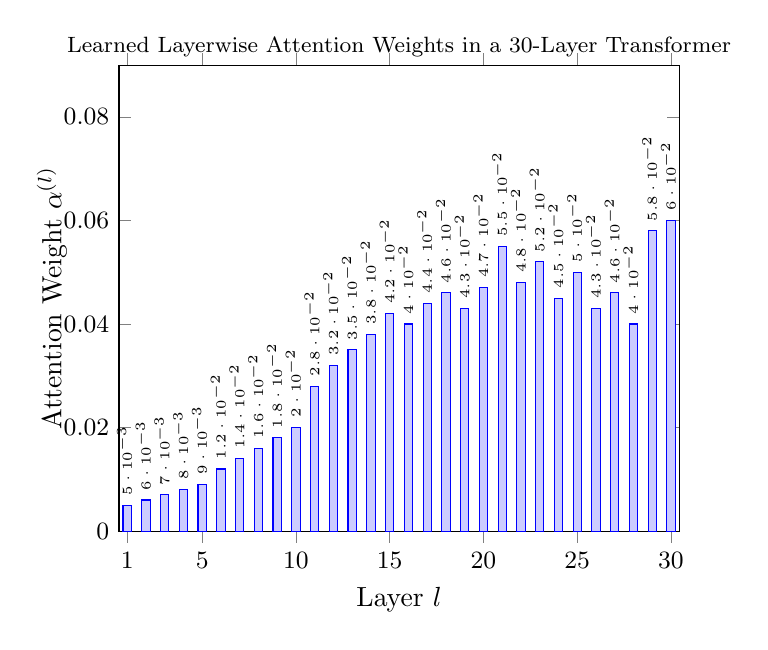
\begin{tikzpicture}
\begin{axis}[
    height=7.5cm,
    ybar,
    ylabel={Attention Weight \(\alpha^{(l)}\)},
    ylabel style={yshift=-8pt},
    xlabel={Layer \(l\)},
    xtick={1,5,10,15,20,25,30},
    ymin=0, ymax=0.09,
    ytick={0,0.02,0.04,0.06,0.08},
    yticklabel style={/pgf/number format/fixed, font=\small},
    bar width=3pt,
    nodes near coords,
    every node near coord/.append style={
        rotate=90,
        anchor=west,
        yshift=1pt,
        font=\tiny,
        color=black
    },
    title style={align=center, yshift=-1.5ex},
    title={\footnotesize Learned Layerwise Attention Weights in a 30-Layer Transformer},
    enlarge x limits=0.015,
    scaled y ticks=false,
    tick label style={font=\small}
]
\addplot[draw=blue, fill=blue!20] coordinates {
    (1,0.005) (2,0.006) (3,0.007) (4,0.008) (5,0.009)
    (6,0.012) (7,0.014) (8,0.016) (9,0.018) (10,0.020)
    (11,0.028) (12,0.032) (13,0.035) (14,0.038) (15,0.042)
    (16,0.040) (17,0.044) (18,0.046) (19,0.043) (20,0.047)
    (21,0.055) (22,0.048) (23,0.052) (24,0.045) (25,0.050)
    (26,0.043) (27,0.046) (28,0.040) (29,0.058) (30,0.060)
};
\end{axis}
\end{tikzpicture}
\end{adjustbox}
\vspace{-4mm}
\caption{
\textbf{Learned Layerwise Pooling Profile.}
The learned attention weights \(\alpha^{(l)}\) peak in mid-depth layers (12--20), where alignment-critical abstractions such as refusal and intent emerge~\cite{belrose2023language, liu2023lost}. Early layers contribute little, while final layers show erratic, low weights, suggesting alignment signals are distributed across depth, not confined to surface activations.
}
\label{fig:layer_attention_varied_random2}
\vspace{-6mm}
\end{figure}





%\paragraph{Outcome.} The resulting pooled vector $\tilde{h}(x, y)$ embeds behavioral geometry—structuring the latent space such that safe completions form a compact submanifold. At the same time, adversarial behaviors collapse into a separable basin. This representation underpins all downstream alignment modules.


\begin{figure*}[ht!]
\vspace{-5mm}
\centering
\begin{tcolorbox}[
  enhanced,
  colback=white,
  colframe=black,
  boxrule=0.8pt,
  borderline={0.6pt}{1.6pt}{black},
  sharp corners,
  width=0.99\textwidth,
  left=2pt,
  right=2pt,
  top=2pt,
  bottom=1pt
]
\tiny
\[
\begin{aligned}
\min_{\theta,\, \alpha^{(l)}} \quad &
\underbrace{
-\log \sigma\left(
\log \pi_\theta(\tilde{h}_{\mathrm{safe}} \mid x)
- \log \pi_\theta(\tilde{h}_{\mathrm{adv}} \mid x)
- \alpha \cdot \left[
\log \pi_{\mathrm{ref}}(\tilde{h}_{\mathrm{safe}} \mid x)
- \log \pi_{\mathrm{ref}}(\tilde{h}_{\mathrm{adv}} \mid x)
\right]
\right)
}_{\textbf{(1) Preference Alignment in Latent Space}} \\[-1pt]
&+ \lambda_{\mathrm{sep}} \cdot
\underbrace{
\left[
\max\left(0,\; M - \left\| \tilde{h}_{\mathrm{safe}} - \tilde{h}_{\mathrm{unsafe}} \right\|_2 \right)
+
\max\left(0,\; M - \left\| \tilde{h}_{\mathrm{safe}} - \tilde{h}_{\mathrm{jb}} \right\|_2 \right)
\right]
}_{\textbf{(2) Safe–Adversarial Separation}} \\[-1pt]
&+ \lambda_{\mathrm{merge}} \cdot
\underbrace{
\max\left(0,\; \left\| \tilde{h}_{\mathrm{unsafe}} - \tilde{h}_{\mathrm{jb}} \right\|_2 - \delta \right)
}_{\textbf{(3) Unsafe–Jailbreak Cohesion}}
\end{aligned}
\]
\end{tcolorbox}
\vspace{-3mm}
\caption{
\textbf{Final GRACE Objective: Preference-Guided Geometric Alignment with Learned Layerwise Pooling.}
This figure presents the complete GRACE loss, which unifies behavior-level preference modeling and latent-space regularization using \emph{learned pooled representations}. The optimization operates over structured triplets—\textbf{safe}, \textbf{unsafe}, and \textbf{jailbreak} responses—and is composed of three interconnected components:
\textbf{(1) Relaxed Preference Loss:}  a DPO-style loss on pooled embeddings \(\tilde{h}_y = \sum_l \alpha^{(l)} h_y^{(l)}\),
\textbf{(2) Latent Separation Loss:} a separation loss enforcing a margin between safe and adversarial completions, and
\textbf{(3) Latent Merging Loss:} a merging loss clustering unsafe and jailbreak behaviors into a shared latent basin.
All components operate over a learned layerwise pooling profile \(\alpha^{(l)}\), enabling behavior-sensitive aggregation without modifying the base LLM. Gradients flow only through the alignment head and pooling weights, embedding alignment structurally within the model's internal geometry.
}
\label{fig:final_objective_geometric_dpo}
\vspace{-4mm}
\end{figure*}


\textbf{Latent Embedding Utility.} 
The pooled representation $\tilde{h}(x, y)$ encodes behavioral geometry—forming a compact submanifold for safe completions while isolating adversarial ones into a separable basin. This latent embedding becomes the universal input to all downstream modules: preference alignment ($\mathcal{L}_{\text{pref}}$), adversarial vulnerability diagnostics (AVQI), and geometric regularization (GRACE). It anchors alignment in latent space, enabling structure-aware safety beyond token-level heuristics. For attention profiles and implementation details, see Appendix; cf. Figure~\ref{fig:layer_attention_varied_random2}.








\section{\textsc{GRACE}: \underline{G}eometric \underline{R}epresentation-\underline{A}ware \underline{C}ontrastive \underline{E}nhancement}
\label{sec:grace_main}

While methods like DPO~\cite{rafailov2023direct} have improved LLM alignment via preference modeling, they act solely at the output level—failing to regulate how safe and unsafe behaviors are represented internally. This blind spot invites \emph{adversarial camouflage}~\cite{turpin2023llms, carlini2023extracting}, where unsafe completions mimic the latent geometry of safe ones, evading refusal filters.

We propose \textsc{GRACE}, a latent-space extension of DPO that reframes alignment as a geometric problem. Rather than relying on final-layer logits, it constructs pooled embeddings \(\tilde{h}_y = \sum_l \alpha^{(l)} h_y^{(l)}\) via a learned layerwise attention profile (cf.~Appendix~\ref{sec:appendix_pool_profile}, Figure~\ref{fig:layer_attention_varied_random2}). These embeddings are shared across all alignment losses, forming a unified latent representation.

The GRACE objective integrates three components: \textbf{(i)} a relaxed preference loss over \(\tilde{h}_y\), encouraging alignment in latent space; \textbf{(ii)} a separation loss that pushes safe completions away from adversarial ones; and \textbf{(iii)} a merging loss that collapses unsafe and jailbreak completions into a compact subspace. All gradients are confined to \(\pi_\theta\) and \(\alpha^{(l)}\); the base LLM remains frozen. GRACE is trained on data as shown in Table~\ref{tab:pairwise-dpo-example}.

Resulting gains include up to \textbf{39\%} ASR reduction (cf. Figure~\ref{fig:grace_benchmark}), with cluster separation illustrated in Figure~\ref{fig:multiview_aqi_comparison}. See Figure~\ref{fig:final_objective_geometric_dpo} for characterization of the full loss and Appendix~\ref{sec:appendix_pool_profile} for further details.










































